\documentclass[12pt,a4paper]{article}
\usepackage{graphicx}
\usepackage{gensymb}
\usepackage{amsmath}
\usepackage{bm}
\usepackage{tikz}
\usepackage{titlesec}
\usepackage{float}

\setcounter{secnumdepth}{4}
\tikzset{
    node distance=2cm, % specifies the minimum distance between two nodes. Change if necessary.
    }
\title{Case Study Modelling an Electronic Component}
\author{
  Azure Hutchings
  \and
  Jean-Luc Danoy
  \and
  Faris Saad S Alsubaie
}
\date{28 October 2019}
 
\begin{document}
 
\begin{titlepage}
\maketitle
\end{titlepage}

\renewcommand{\abstractname}{Executive Summary}
\begin{abstract}
Write Abstract Here
\end{abstract}

\pagebreak

\tableofcontents

\pagebreak

\section{Introduction}

\subsection{Purpose of the Report}
The following report investigates the steady-state heat distribution in a newly designed component. 

The report will discuss how to numerically solve for the steady-state heat distribution, the efficient of different methods and the effect of different ambient temperatures.

\subsection{The Maths of the Problem}

\begin{figure}[H]
	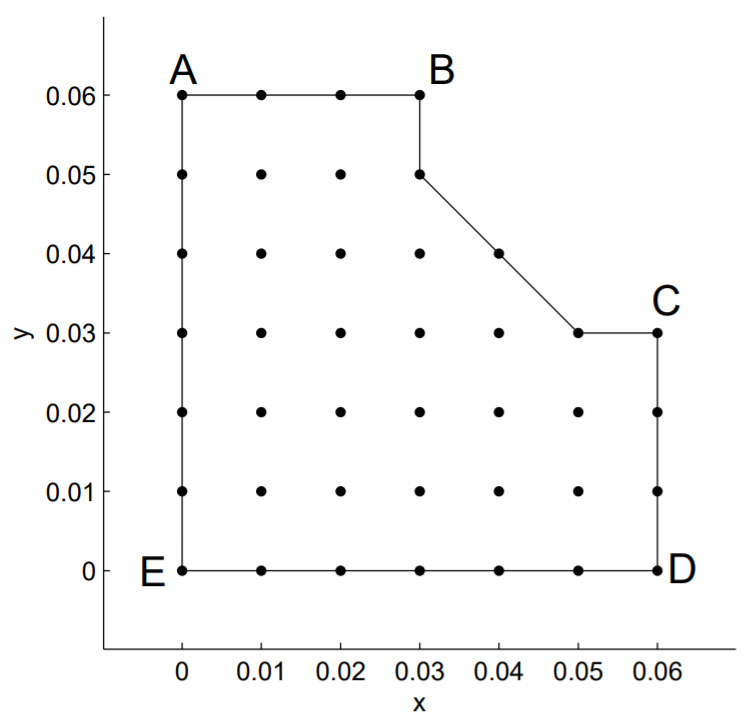
\includegraphics[width=\linewidth]{images/Component.png}
	\caption{Schematic of electronic component.}
	\label{fig:componentSchematic}
\end{figure}

The component schematic is shown in Figure \ref{fig:componentSchematic}. The location of the component within the device means it's subject to different temperature condition along it's boundaries. The boundary A-B is in perfect thermal contact with another component which the temperature is known to 70\degree C. The boundary C-D is also in perfect thermal contact with another component which the temperature is known to be 40\degree C. The boundary A-E-D is thermally insulated and the boundary B-C is exposed to the air at ambient temperature.
\\\\
This type of model can be described with Laplace's equation. Letting $T(x,y)$ represent the temperature of the component at point $(x, y)$, the model is as follows	

\begin{center}
\begin{tabular}{c c}
$\frac{\partial^2 T}{\partial x^2}+\frac{\partial^2 T}{\partial y^2}=0$ & in the interior\\
$T = 70$ & on boundary A-B \\
$T = 40$ & on boundary C-D \\
$\boldsymbol{\nabla} T \cdot {\hat{\textbf{n}}} = 0$ & on boundary A-E-D\\
$k\boldsymbol{\nabla}T\cdot\hat{\textbf{n}} = h(T_{\infty} - T)$ & on boundary B-C
\end{tabular}
\end{center}
Where the thermal conductivity is $k=3Wm^{-1}C^{-1}$, and the heat transfer coefficient is $h=20 Wm^{-2}C^{-1}$. To begin with, we will assume the ambient temperature is $T_\infty = 20$.
\clearpage
\section{Method for Discretising the Problem}
If this was left as a continuous partial differential equation, we would need to analytically solve it. However, it can be much quicker to numerically solve this problem and still retain a high degree of accuracy with the final answers. In this section we will show how we converted the analytical problem to a numerical problem, how the mesh was constructed, the node ordering used, the linear system we derived from the mesh and discuss the matrix that was created from it.


\subsection{Constructing the Finite Difference Mesh}
Suppose we had a function $\phi(x,y,t)$ which gives the temperature at the point (x,y) on a 2-dimensional plane where t is the time since the start of the initial conditions. If the function has a steady-state solution, then it means at some point in time, any increase in time will not result in a change of temperature. This means that 
\begin{center}
$\frac{d\phi}{dx}|_{x_i}\approx\frac{\phi(x_i+\Delta x)-\phi(x_i)}{\Delta x}$,
\end{center}
where the change in $x$ along $\phi$ at the point $x_i$ is approximately the functions forward difference over the distance between nodes. We can then take the derivative of this again using backwards difference to get the second derivative centred around $x_i$.
\begin{center}
$\frac{d^2\phi}{dx^2}|_{x_i}\approx\frac{\phi(x_i+\Delta x)-2\phi(x_i)+\phi(x_i-\Delta x)}{(\Delta x)^2}$,
\end{center}
If we do the same for the change in $y$, we arrive at an analogous equation
\begin{center}
$\frac{d^2\phi}{dy^2}|_{y_i}\approx\frac{\phi(y_i+\Delta y)-2\phi(y_i)+\phi(y_i-\Delta y)}{(\Delta y)^2}$,
\end{center}
To numerically solve this problem, a finite difference mesh must be constructed and a matrix must be created to represent this information.
\\
By splitting the component up into intervals of 0.01 in both the $x$ and $y$ direction, the component can be split into a $7 \times 7$ grid. Because we know that the temperature on the upper and right hand boundaries are fixed temperatures, we can ignore them in our discretisation as nodes. They will come into effect later as the right hand side matrix. Given the previous mesh from the introduction, we can label each node u$_{i,j}$ for $i,j = 0$ to 6 where $i, j$ are given by the row and column of the node starting from the bottom left hand corner. Replacing $\phi(x,y,t)$ with $u_{i,j}(t)$ and noting that $\Delta x = \Delta y$, we arrive at the set of equations for the change in $u_{i,j}(t)$.
\begin{center}
$u'_{i,j}(t)\approx\frac{D}{\Delta x^2}\big{(}-u_{i+1,j}(t)-u_{i,j+1}(t)+4u_{i,j}(t)-u_{i-1,j}(t)-u_{i,j-1}(t)\big{)}.$
\end{center}
Note that since we are finding a state where the temperature does not change in time $(u'_{i,j}(t)=0)$, and assuming that $D\neq0$, we can rewrite this to be
\begin{center}
  $0=\big{(}-u_{i+1,j}-u_{i,j+1}+4u_{i,j}-u_{i-1,j}-u_{i,j-1}\big{)}.$
\end{center}
There are 3 different types of mesh that need to be created. These are for the A-E-D boundary, the interior of the mesh, and on the B-C boundary.
\subsubsection{Interior Nodes}
On the interior of the mesh, each node contains 4 other nodes adjacent to it, and the change in temperature at that node is given by the equation
\begin{center}
\[\frac{\partial^2 T}{\partial x^2}+\frac{\partial^2 T}{\partial y^2}=0\]
\[\frac{2T-T_W-T_E}{(0.01)^2}+\frac{2T-T_N-T_S}{(0.01)^2}=0\]
\[4T-T_W-T_E-T_N-T_S=0\]
\end{center}
\begin{center}
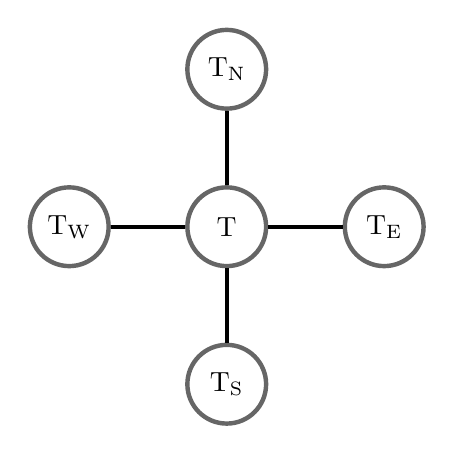
\begin{tikzpicture}[
roundnode/.style={circle, draw=black!60, ultra thick,  minimum size=10mm},
]
\node[roundnode] (center) {T};
\node[roundnode] (left) [left of=center] {T$_\text{W}$};
\node[roundnode] (right) [right of=center] {T$_\text{E}$};
\node[roundnode] (above) [above of=center] {T$_\text{N}$};
\node[roundnode] (below) [below of=center] {T$_\text{S}$};

\draw[ultra thick,-] (left.east) -- (center.west);
\draw[ultra thick,-] (above.south) -- (center.north);
\draw[ultra thick,-] (right.west) -- (center.east);
\draw[ultra thick,-] (below.north) -- (center.south);
\end{tikzpicture}
\end{center}
As an example, the node $T_{(1,1)}$ can be examined.
\begin{center}
  $4T_{(1,1)}-T_{(0,1)}-T_{(2,1)}-T_{(1,2)}-T_{(1,0)}=0$
\end{center}
\subsubsection*{Boundary A-E-D Nodes}
On the boundary A-E-D, there are no nodes outside of the matrix. We can approximate them using first order forward differences (to keep the A matrix SPD). This approximation can be done using the rule $\boldsymbol{\nabla} T \cdot {\hat{\textbf{n}}} = 0$, where ${\hat{\textbf{n}}}$ is the normal unit vector at the node T and $\boldsymbol{\nabla} T$ is the directional gradient at T. The first order differences are then used to construct a finite difference equations for each node on the boundary.\\We will provide 3 examples that show all the unique cases along the boundary A-E-D, namely on the border A-E (not including A or E), the border E-D (not including E or D) and the node E.
\paragraph*{Nodes A-E}
On the A-E nodes, the normal unit vector will face directly west.
\begin{center}
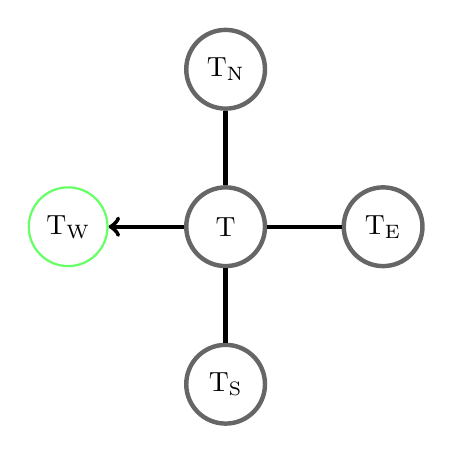
\begin{tikzpicture}[
roundnode/.style={circle, draw=black!60, ultra thick,  minimum size=10mm},
ghostnode/.style={circle, draw=green!60, thick, minimum size = 10mm},
]
\node[roundnode] (center) {T};
\node[ghostnode] (left) [left of=center] {T$_\text{W}$};
\node[roundnode] (right) [right of=center] {T$_\text{E}$};
\node[roundnode] (above) [above of=center] {T$_\text{N}$};
\node[roundnode] (below) [below of=center] {T$_\text{S}$};

\draw[ultra thick,<-] (left.east) -- (center.west);
\draw[ultra thick,-] (above.south) -- (center.north);
\draw[ultra thick,-] (right.west) -- (center.east);
\draw[ultra thick,-] (below.north) -- (center.south);
\end{tikzpicture}
\end{center}
Therefore $\hat{\textbf{n}} = (-1,0)^T$. We can construct a first order forward difference approximation for $T_W$.
\begin{center}
\[\bigg{(}\frac{\partial T}{\partial x},\frac{\partial T}{\partial y}\bigg{)}\cdot (-1,0)^T = 0\]
\[-\frac{\partial T}{\partial x} = 0\]
\[\frac{T-T_W}{0.01} = 0\]
\[T_W = T.\]
\end{center}
This value of $T_W$ can be used in the stencil around the point T.
\begin{center}
\[\frac{\partial^2 T}{\partial x^2}+\frac{\partial^2 T}{\partial y^2}=0\]
\[\frac{2T-T_W-T_E}{(0.01)^2}+\frac{2T-T_N-T_S}{(0.01)^2}=0\]
\[2T-T_W-T_E+2T-T_N-T_S=0\]
\[4T-T-T_E-T_N-T_S=0\]
\[3T-T_E-T_N-T_S=0.\]
\end{center}

As an example, let's look at node $T_{(0, 3)}$. 
\begin{center}
  $3T_{(0,3)}-T_{(1,3)}-T_{(0,4)}-T_{(0,2)}=0$
\end{center}

\paragraph*{The Node E:}
On the node E, or (0,0) the unit normal vector will be facing south-west.
\begin{center}
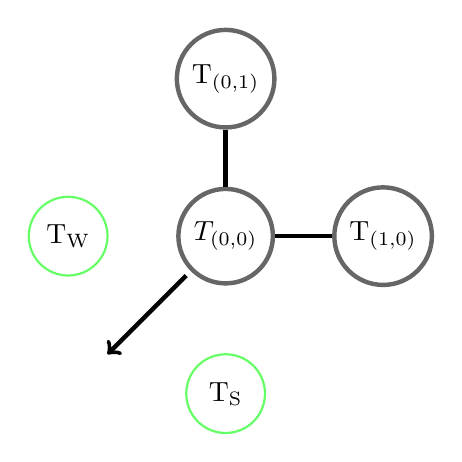
\begin{tikzpicture}[
roundnode/.style={circle, draw=black!60, ultra thick,  minimum size=10mm},
ghostnode/.style={circle, draw=green!60, thick, minimum size = 10mm},
]
\node[roundnode] (center) {$T_{(0,0)}$};
\node[ghostnode] (left) [left of=center] {T$_\text{W}$};
\node[roundnode] (right) [right of=center] {T$_{(1,0)}$};
\node[roundnode] (above) [above of=center] {T$_{(0,1)}$};
\node[ghostnode] (below) [below of=center] {T$_\text{S}$};


\draw[ultra thick,-] (above.south) -- (center.north);
\draw[ultra thick,-] (right.west) -- (center.east);
\draw[ultra thick,->] (-0.5,-0.5) -- (-1.5,-1.5);

\end{tikzpicture}
\end{center}
As a normalised vector, it will be 
\begin{center}
    $\hat{\textbf{n}} = \frac{1}{\sqrt{2}}(-1,-1)^T$.
\end{center}
We can use this in our boundary condition to create a first order difference approximation for $T_W + T_S$.
\begin{center}
  \[\bigg{(}\frac{\partial T}{\partial x},\frac{\partial T}{\partial y}\bigg{)}\cdot \frac{1}{\sqrt{2}}(-1,-1)^T = 0\]
  \[\bigg{(}\frac{\partial T}{\partial x},\frac{\partial T}{\partial y}\bigg{)}\cdot (-1,-1)^T = 0\]
  \[\bigg{(}\frac{\partial T}{\partial x}+\frac{\partial T}{\partial y}\bigg{)} = 0\]
  \[\frac{T-T_W}{0.01}+\frac{T-T_S}{0.01} = 0\]
  \[T_W+T_S=2T.\]
\end{center}
Substituting this into our stencil, we can see that 
\begin{center}
\[4T_{(0,0)}-T_{(0,1)}-T_{(1,0)}-T_{W}-T{S}=0\]
\[4T_{(0,0)}-T_{(0,1)}-T_{(1,0)}-2T_{(0,0)}=0\]
\[2T_{(0,0)}-T_{(0,1)}-T_{(1,0)}=0.\]
\end{center}

\paragraph*{Nodes E-D:} On the nodes E-D, the normal unit vector will face directly south. 
\begin{center}
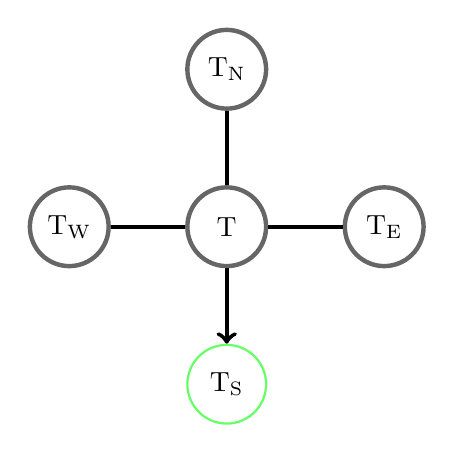
\begin{tikzpicture}[
roundnode/.style={circle, draw=black!60, ultra thick,  minimum size=10mm},
ghostnode/.style={circle, draw=green!60, thick, minimum size = 10mm},
]
\node[roundnode] (center) {T};
\node[roundnode] (left) [left of=center] {T$_\text{W}$};
\node[roundnode] (right) [right of=center] {T$_\text{E}$};
\node[roundnode] (above) [above of=center] {T$_\text{N}$};
\node[ghostnode] (below) [below of=center] {T$_\text{S}$};

\draw[ultra thick,-] (left.east) -- (center.west);
\draw[ultra thick,-] (above.south) -- (center.north);
\draw[ultra thick,-] (right.west) -- (center.east);
\draw[ultra thick,<-] (below.north) -- (center.south);
\end{tikzpicture}
\end{center}
This can be written as 
\begin{center}
  $\hat{\textbf{n}}=(0,-1)^T$.
\end{center}
Using the same boundary rule for the edge A-E-D (which contains the edge E-D) we can find a first order forward difference for $T_S$.
\begin{center}
\[\bigg{(}\frac{\partial T}{\partial x},\frac{\partial T}{\partial y}\bigg{)}\cdot (0,-1)^T = 0\]
\[-\frac{\partial T}{\partial y}=0\]
\[\frac{T-T_S}{0.01}=0\]
\[T_S=T\]
\end{center} 
Using this in our finite difference equation, we get the following equation for a node along the boundary E-D.
\begin{center}
  \[4T-T_S-T_N-T_W-T_E=0\]
  \[4T-T-T_N-T_W-T_E=0\]
  \[3T-T_N-T_W-T_E=0.\]
\end{center}
As an example, let us look at node $T_{(3,0)}$.
\begin{center}
  $3T_{(3,0)}-T_{(3,1)}-T_{(2,0)}-T_{(4,0)}=0$.
\end{center}
Each other node along the boundary will be similar to this node.
\subsubsection*{Boundary B-C}
There are three nodes that we care about on the boundary B-C. These are nodes (3,5), (4,4) and (5,3). Each of these nodes will have a different normal vector and so must all be calculated individually. However, they all have the same boundary condition 
\[k\boldsymbol{\nabla}T\cdot\hat{\textbf{n}} = h(T_{\infty} - T).\]
\paragraph*{Node (3,5):} At this node, the normal vector is going to be facing directly east. This can be seen by analysing the mesh around the point $T_{(3,5)}$.
\begin{center}
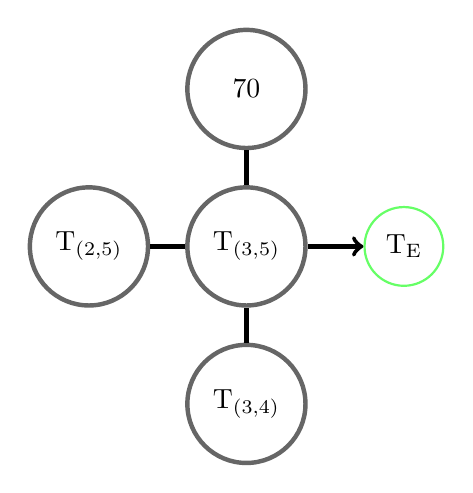
\begin{tikzpicture}[
roundnode/.style={circle, draw=black!60, ultra thick,  minimum size=15mm},
ghostnode/.style={circle, draw=green!60, thick, minimum size = 10mm},
]
\node[roundnode] (center) {T$_{(3,5)}$};
\node[roundnode] (left) [left of=center] {T$_\text{(2,5)}$};
\node[ghostnode] (right) [right of=center] {T$_\text{E}$};
\node[roundnode] (above) [above of=center] {70};
\node[roundnode] (below) [below of=center] {T$_\text{(3,4)}$};

\draw[ultra thick,-] (left.east) -- (center.west);
\draw[ultra thick,-] (above.south) -- (center.north);
\draw[ultra thick,<-] (right.west) -- (center.east);
\draw[ultra thick,-] (below.north) -- (center.south);
\end{tikzpicture}
\end{center}
Therefore the normal unit vector is 
\begin{center}
  $\hat{\textbf{n}}=(1,0)^T$.
\end{center}
A first order backward difference is used here because the node we are estimating, T$_\text{E}$, is to the right of the node T$_{(3,5)}$.
\[
  k\boldsymbol{\nabla}T_{(3,5)}\cdot(1,0)^T = h(T_{\infty} - T_{(3,5)})
\]
\[ 3\bigg{(}\frac{\partial T_{(3,5)}}{\partial x},\frac{\partial T_{(3,5)}}{\partial y}\bigg{)}\cdot(1,0)^T = 20(20 - T_{(3,5)})\]
\[3\frac{T_E-T_{(3,5)}}{0.01} = 400-20T_{(3,5)}\]
\[3T_E-3T_{(3,5)}=4-0.2T_{(3,5)}\]
\[T_E=\frac{4}{3}+\frac{2.8}{3}T_{(3,5)}.\]
The second order central difference at T$_{(3,5)}$ will therefore be 
\[4T_{(3,5)}-T_N-T_S-T_W-T_E=0\]
\[4T_{(3,5)}-70-T_{(3,4)}-T_{(2,5)}-\bigg{(}\frac{4}{3}+\frac{2.8}{3}T_{(3,5)}\bigg{)}=0\]
\[\frac{9.2}{3}T_{(3,5)}-T_{(3,4)}-T_{(2,5)}=70+\frac{4}{3}.\]
\paragraph*{Node (5,3):} The case at this node is isomorphic to the node at (3,5), as $\Delta x = \Delta y$ and the normal vector is $(0,1)^T$ rather than $(1,0)^T$. So instead of getting a value for T$_E$ in terms of T$_{(3,5)}$, we will get a value for T$_S$ in terms of T$_{(5,3)}$ for the boundary condition.
\[T_S=\frac{4}{3}+\frac{2.8}{3}T_{(5,3)}.\]
Substituting this in our second order central difference for T$_{(5,3)}$ yeilds
\[4T_{(5,3)}-T_N-T_S-T_W-T_E=0\]
\[4T_{(5,3)}-\bigg{(}\frac{4}{3}+\frac{2.8}{3}T_{(5,3)}\bigg{)}-T_{(5,2)}-T_{(4,3)}-40=0\]
\[\frac{9.2}{3}T_{(5,3)}-T_{(5,2)}-T_{(4,3)}=40+\frac{4}{3}.\]
\subsection{Node Ordering}
One last thing we must do is construct a mapping from the 2D array of nodes to a 1D array of nodes. This is useful when creating the vectors $x$ and $b$ in the linear equation $Ax=b$.
\\
Because we have a $6 \times 6$ array (ignoring the missing or null nodes in the top right corner) we can transform this into a 1D array with 36 values. We can use the following assumptions to construct the map \begin{itemize}
\item Our index is $(i,j)$ with $i$ being the horizontal coordinate and $j$ being the vertical coordinate 
\item (0,0) is the bottom left node 
\item ($i+1$,$j$) is to the right of ($i$,$j$) and ($i$,$j+1$) is above ($i$,$j$)
\end{itemize}
From this we can deduce that every time we move across the 2D array, we are moving 1 unit across in the 1D array, and every time we move up in the 2D array, we are moving 6 across in the 1D array. Therefore,
\begin{center}
$(i,j) \to i+6j$.
\end{center}

\subsection{Matrix Construction}
%\subsection{Research methods}
%
%
%\subsection{Limitations and assumptions}
%

\section{Discussion}

\subsection{Efficiency Comparison}
The following section investigates which numerical method or methods provide the greatest efficiency in solving problems similar to the electronic component.

\subsubsection{Bandwidth and level of fill-in for Each Different Node Ordering}


\subsubsection{Memory (for Direct Methods)}
\begin{center}
\begin{tabular}{c c c c c}
Name & Size & Bytes & Class & Attributes \\
\hline
$A$ & $33 \times 33$ & $8712$ & double & \\
$A$ Banded Storage & $33 \times 7$ & $1848$ & double & \\
$A$ Packed Storage & $1 \times 561$ & $4488$ & double & \\
$A$ Sparse Storage & $33 \times 33$ & $2528$ & double & sparse \\
$b$ & $33 \times 1$ & $264$ & double & \\
\end{tabular}
\end{center}

\begin{figure}[H]
	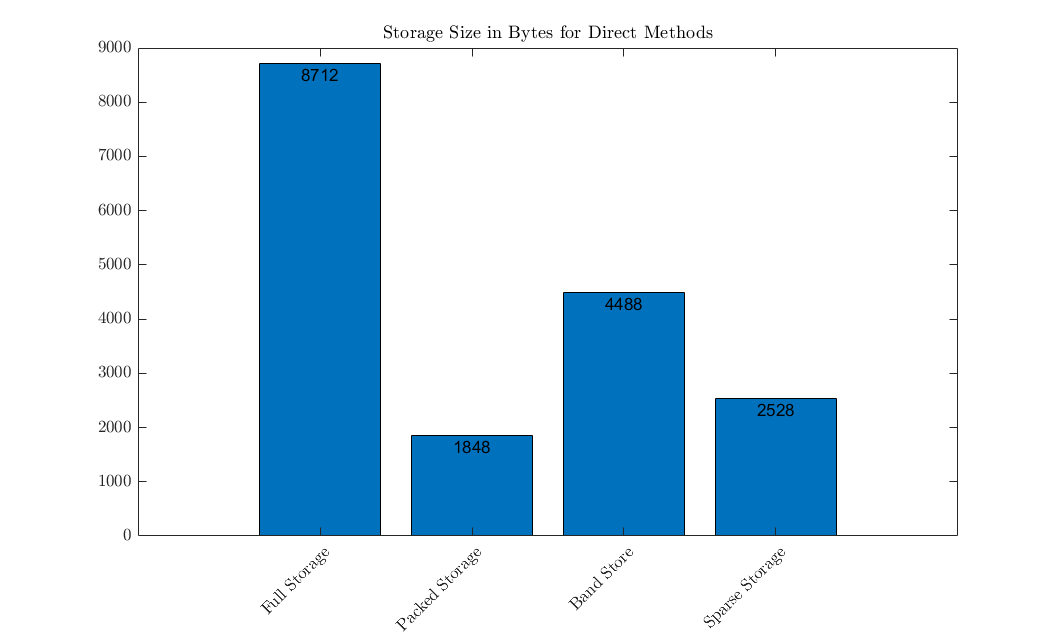
\includegraphics[width=\linewidth]{images/MemoryGraph.png}
	\caption{Memory of each of the A and b which are stored for each Direct Method.}
	\label{fig:memory}
\end{figure}

\subsubsection{Iterations (for Iterative Methods)}
\begin{figure}[H]
	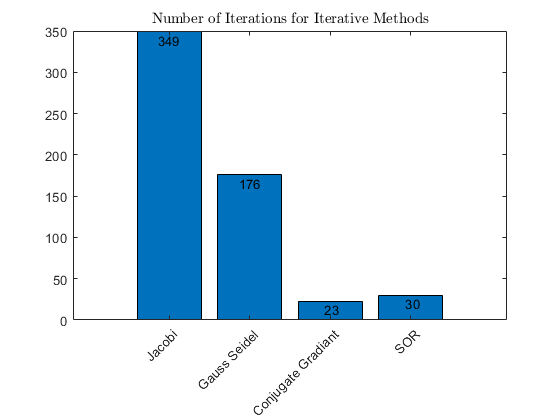
\includegraphics[width=\linewidth]{images/IterationsGraph.png}
	\caption{Number of Iterations for each Iterative Method}
	\label{fig:iterations}
\end{figure}


\subsubsection{Runtime (Direct and Iterative)}
\begin{figure}[H]
	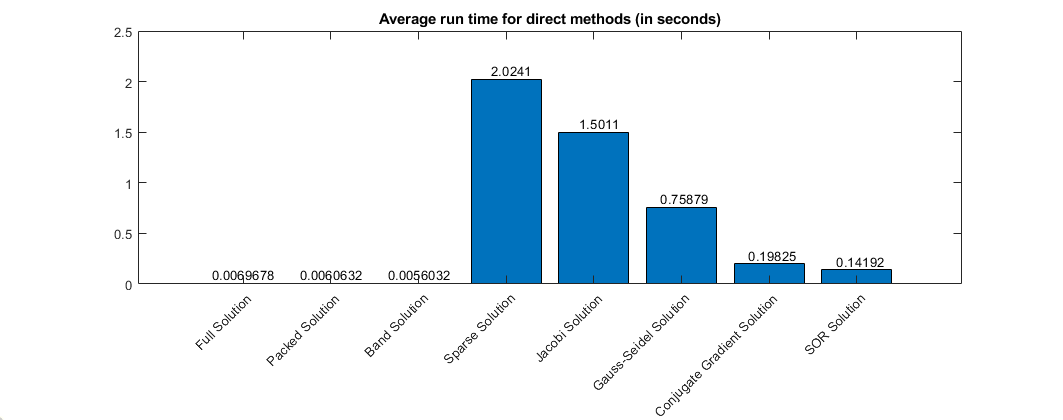
\includegraphics[width=\linewidth]{images/RuntimeGraph.png}
	\caption{Runtime for solving each of the Direct and Iterative Methods.}
	\label{fig:runtime}
\end{figure}

\subsubsection{Floating Point Operations (Direct and Iterative)}
\begin{figure}[H]
	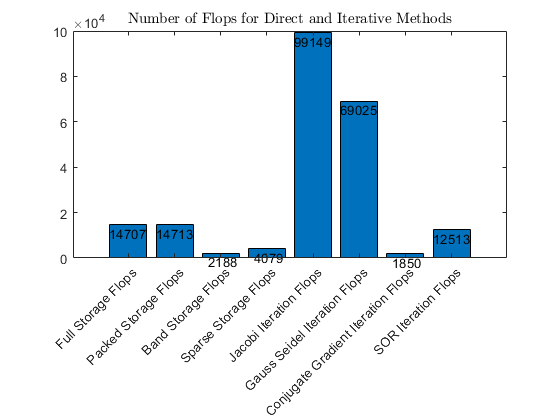
\includegraphics[width=\linewidth]{images/FlopsGraph.png}
	\caption{Flops for each Direct and Iterative Methods.}
	\label{fig:flops}
\end{figure}

\begin{figure}[H]
	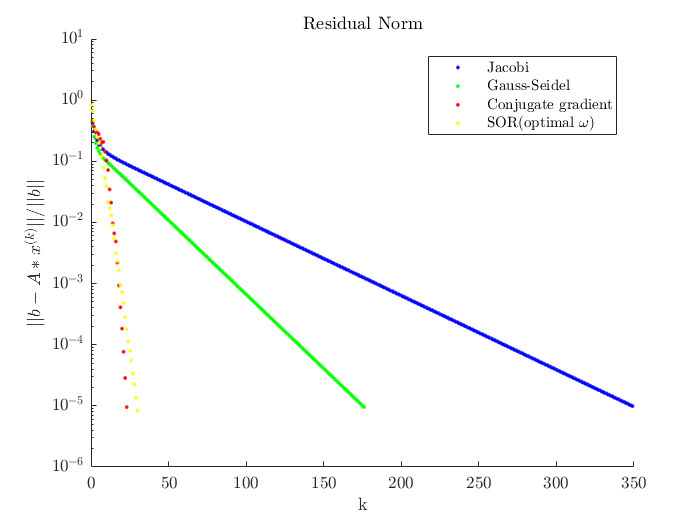
\includegraphics[width=\linewidth]{images/ResidualNormGraph.png}
	\caption{Residual Norm for each Iterative Methods}
	\label{fig:res}
\end{figure}

\subsubsection{Tolerance Required for Iterative Methods)}

\begin{figure}[H]
	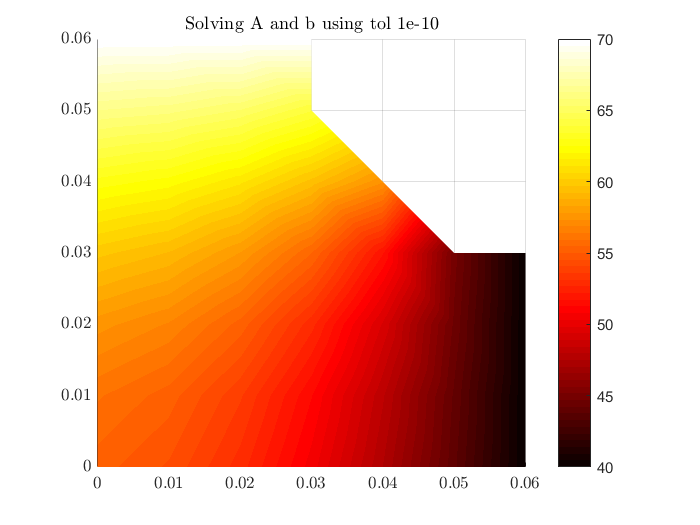
\includegraphics[width=\linewidth]{images/Comparisontole-10.png}
	\caption{Tolerance of $10^{-10}$.}
	\label{fig:tole-10}
\end{figure}

\begin{figure}[H]
	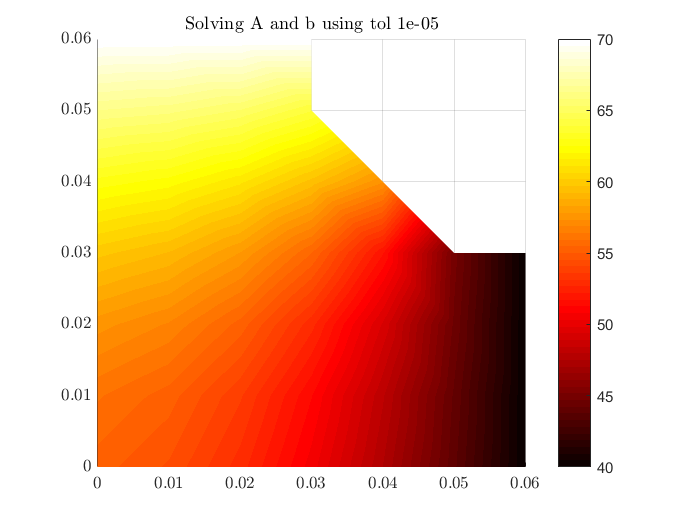
\includegraphics[width=\linewidth]{images/Comparisontole-05.png}
	\caption{Tolerance of $10^{-5}$.}
	\label{fig:tole-05}
\end{figure}

\begin{figure}[H]
	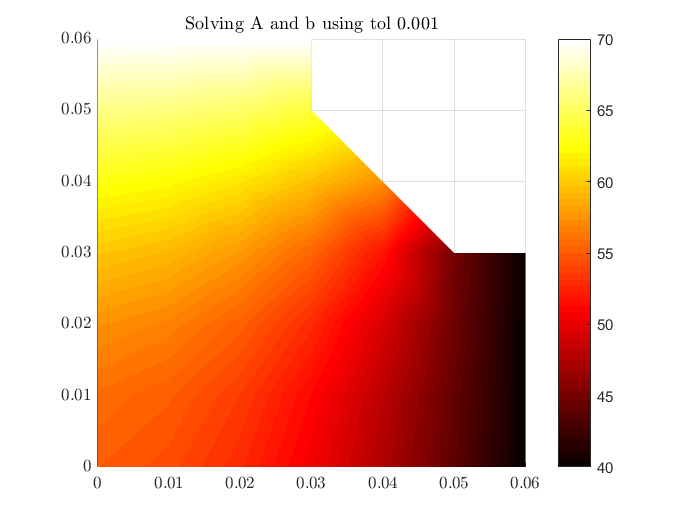
\includegraphics[width=\linewidth]{images/Comparisontol0-001.png}
	\caption{Tolerance of $10^{-3}$.}
	\label{fig:tol0.001}
\end{figure}

\begin{figure}[H]
	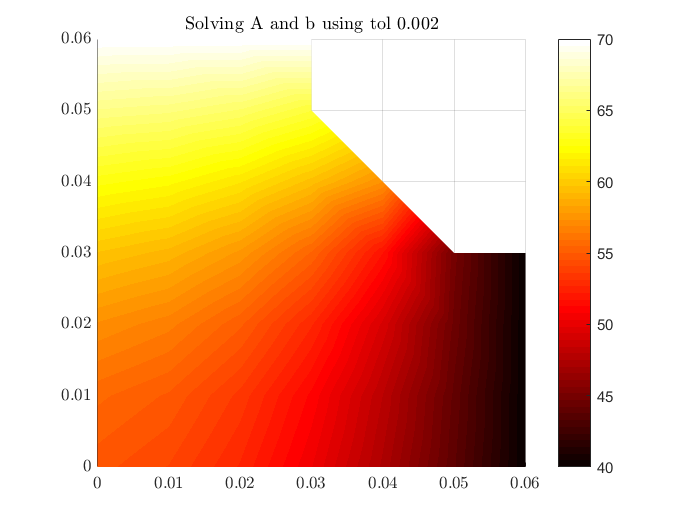
\includegraphics[width=\linewidth]{images/Comparisontol0-002.png}
	\caption{Tolerance of $2 \times 10^{-3}$.}
	\label{fig:tol0.002}
\end{figure}

\begin{figure}[H]
	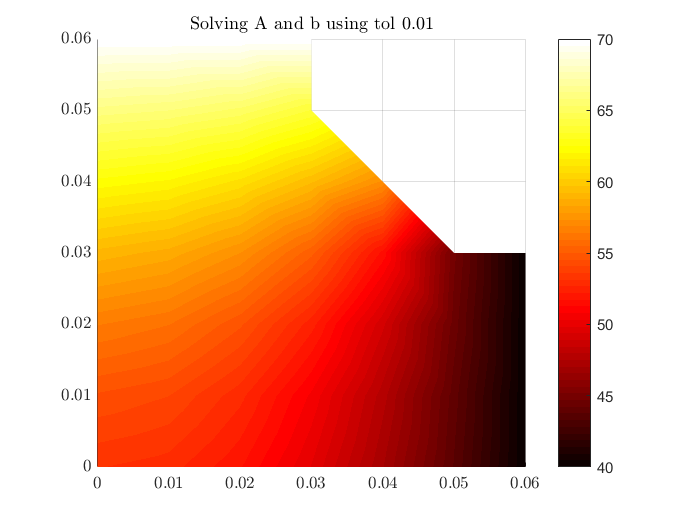
\includegraphics[width=\linewidth]{images/Comparisontol0-01.png}
	\caption{Tolerance of $10^{-2}$.}
	\label{fig:tol0.01}
\end{figure}

\begin{figure}[H]
	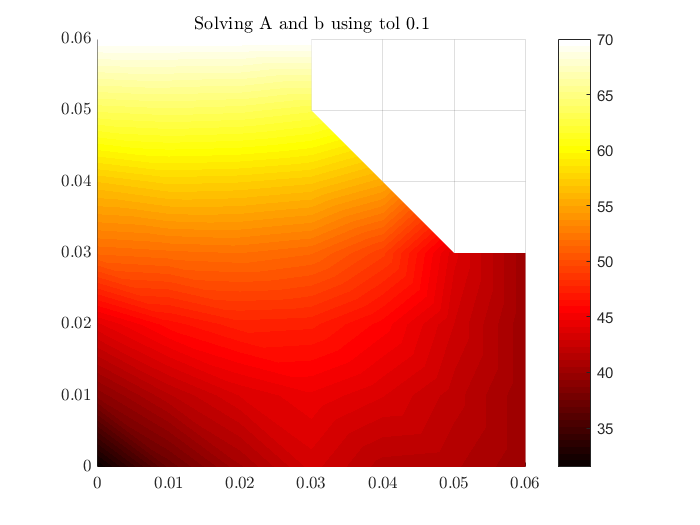
\includegraphics[width=\linewidth]{images/Comparisontol0-1.png}
	\caption{Tolerance of $10^{-1}$.}
	\label{fig:tol0.1}
\end{figure}

\begin{figure}[H]
	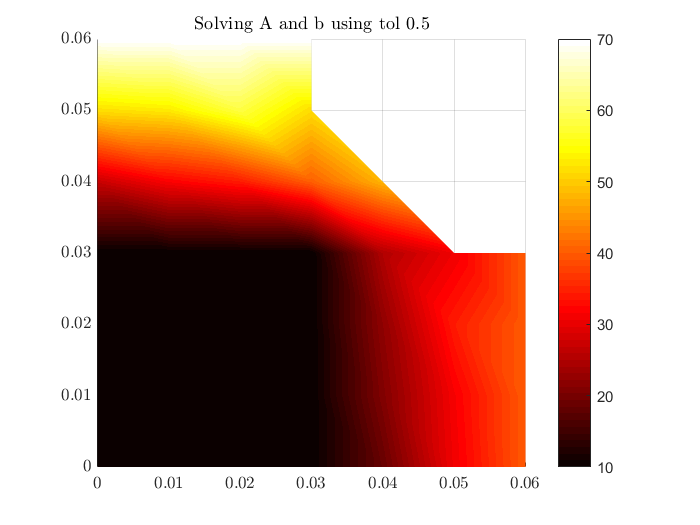
\includegraphics[width=\linewidth]{images/Comparisontol0-5.png}
	\caption{Tolerance of $0.5$.}
	\label{fig:tol0.5}
\end{figure}

\begin{figure}[H]
	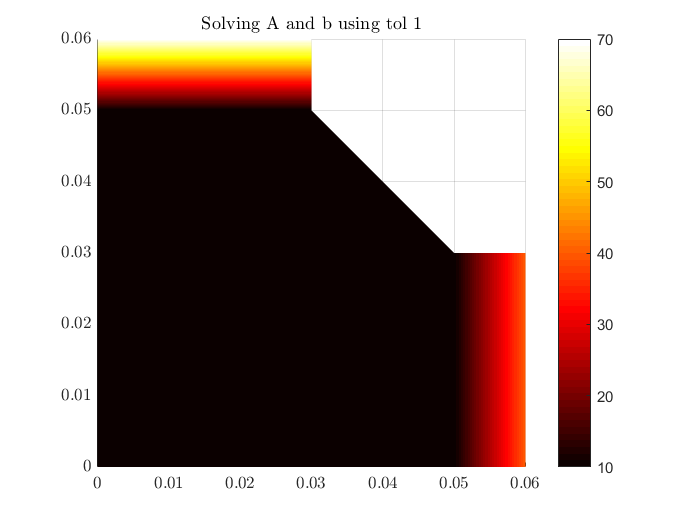
\includegraphics[width=\linewidth]{images/Comparisontol1.png}
	\caption{Tolerance of $1$.}
	\label{fig:tol1}
\end{figure}

\subsubsection{Effect of $\omega$ on the Rate of Convergence of the SOR Method)}
\begin{figure}[H]
	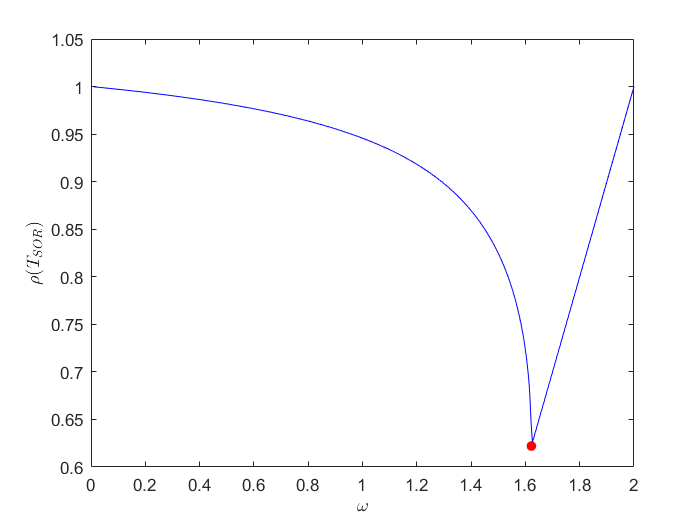
\includegraphics[width=\linewidth]{images/omegaGraph1.png}
	\caption{Omega.}
	\label{fig:omega1}
\end{figure}

\begin{figure}[H]
	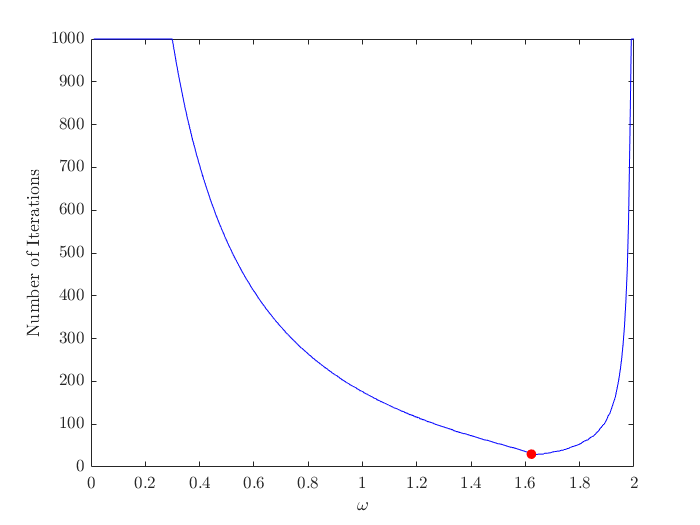
\includegraphics[width=\linewidth]{images/omegaGraph2.png}
	\caption{Number of Iterations against different values of $\omega$.}
	\label{fig:omega2}
\end{figure}

%
%\subsection{Method}
%
%\subsubsection{Procedures}
%
%\subsubsection{Sample Size}
%
%\subsubsection{Selection Criteria}
%
%\subsection{Discussion and analysis of data}
%
%\subsubsection{Issue 1}
%
%\subsubsection{Issue 2}
%
%\subsubsection{Issue 3}
%
%\subsubsection{Reliability and accuracy of data}
%
%\section{Conclusions}
%
%\section{Recommendations}
%
%\subsection{Recommendation 1}
%
%\subsection{Recommendation 2}
%
%\section{References}
%
%\section{Appendices}
 
\end{document}